\chapter{Einleitung}
\label{ch:intro}


\section{Motivation}
\label{ch1:motivation}
% Was ist das Problem?
% Warum ist das ein relevantes Problem?
Die unter Naturschutz stehenden Rotmilanbestände sind in den letzten zwanzig Jahren um 30 Prozent eingebrochen.
Etwa 60 Prozent der Rotmilane sind in Deutschland angesiedelt, daher ergibt sich die Notwendigkeit, diesen Bestand zu erhalten \cite{landesbund_fur_vogelschutz_in_bayern_rotmilan_nodate}.
Von März bis August fliegt der Rotmilan über die Felder rund um die Windräder.
Bei einer Bodenbewirtschaftungsmaßnahme werden diverse Kleintiere aufgescheucht.
Da der Rotmilan bei der Jagd die Ackerflächen nach Kleintieren absucht, achtet er nicht auf mögliche Kollisionen mit Rotorblättern oder Masten vor ihm.
In diesem Kontext gehört der unter Naturschutz stehende Rotmilan zu den am häufigsten betroffenen Vogelarten \cite{grunkorn_ermittlung_2016}.

\bigskip
Untermauert wird das Problem durch ein Expertengespräch \cite{blew_wirksamkeit_2018}, in dem das Abschalten der \ac{WEA} bei Bodenbewirtschaftungsereignissen primär als Maßnahme zur Reduktion der tödlichen Kollisionen bestimmt wurde. \\
In der Regel müssen die Bauern ihre Mahdaktivitäten beim Windparkbetreiber melden.
Dafür gibt es jedoch keine Gewähr.
% Dies erfolgt jedoch unzuverlässig. \TODO{mit geringer gewähr}
Die Landflächen können weiter verpachtet werden und somit von unterschiedlichen Traktoren befahren werden, daher ist das Verbauen von (GPS-) Sensoren am Traktor keine Option.

Deshalb gilt es, automatisiert Traktoren in einem Radius von bis zu \SI{300}{\metre} zu erkennen und zu melden.

Wurde eine Mahdaktivität festgestellt, wird die \ac{WEA} bis zu drei Tage abgeschaltet.
Dabei ist zum jetzigen Stand die einzige Anforderung an die Windparkbetreiber, dass die Kollisionsrate unter eine \textit{Signifikanzschwelle} gesenkt werden muss \cite{schuster_anforderungen_2019} \cite[\S~44]{noauthor_bnatschg_2009}.
% Die genauen Anforderungen für ein fertiges System sind noch nicht bekannt.
% Als Grundlage sollen Traktoren in Bildsequenzen gefunden werden.

\bigskip
Zum Erkennen von Objekten in Bildern werden heute oft Objekt Detektoren wie YOLOv3 \cite{redmon_yolov3:_2018}, Faster R-CNN \cite{ren_faster_2015}, TridentNet \cite{li_scale-aware_2019} oder TrackNet \cite{li_tracknet:_2019} eingesetzt.
Diese erreichen zwar sehr hohe Genauigkeiten, sind jedoch nicht für leistungsschwache Endgeräte ausgelegt \cite{hossain_deep_2019}.
Grund dafür ist unter anderem, dass viele potenzielle Bereiche \IT{(Region Porposals)} abgetastet und klassifiziert werden.
Hinzu kommt, dass hierbei Objekte nur zuverlässig erkannt werden, die eine Größe von mindestens $32px^2$ im Bild einnehmen \cite{wu_recent_2019}.
Die Bilder werden bei diesen Ansätzen typischerweise stark herunterskaliert.
Daher sind Objekte, die vor Skalierung nur knapp die Mindestgröße aufweisen, zu klein.
Das Bild müsste deshalb in mehrere Teile geschnitten werden, was sich zusätzlich negativ auf den Durchsatz auswirken würde.

Die genannten Detektoren bieten sich vor allem für die Analyse starrer Bilder an.
Handelt es sich allerdings um Bildsequenzen, ist dafür ein enormer Ressourcenaufwand notwendig, da jedes einzelne Videobild (Frame) komplett abgetastet werden muss.

\section{Ziel der Arbeit}
% Wie stelle ich mir eine Lösung des Problems vor?
Als Grundlage für ein fertiges System wird in dieser Arbeit das Erkennen der Traktoren in Bildsequenzen untersucht.

Ziel ist die Erkennung in einem Radius von $300$ Metern um das Windrad.
Um den Energiebedarf für die dauerhafte Überwachung möglichst gering zu halten, gilt es einen Ansatz zu entwickeln, welcher auf leistungsschonenden Geräten, wie der \textsc{NVIDIA Jetson} Familie, arbeiten kann.
% \TODO{Preisleistung Günstige Anschaffung + Haltung}

Es soll eine Lösung auf Basis von Machine Learning Techniken entwickelt werden, die Traktoren effizient in Bildsequenzen erkennt.
% Das hier vorgestellte Konzept teilt sich auf in:
% \begin{itemize}
%     \item{\textbf{Background Subtraction}}: Bewegungen im Kamerabild erkennen. Die Bewegungen stellen die sogenannten \acp{ROI} dar.
%     \item{\textbf{\ac{CNN}}}: Klassifizieren, ob es sich bei den gefundenen \ac{ROI} um eine landwirtschaftliche Maschine handelt.
% \end{itemize}

% Mit diesem Konzept sollen Traktoren in Bildsequenzen effektiv erkannt werden.

\section{Methodik und Aufbau}
% Wie will ich vorgehen, um das Problem zu lösen?
Da zur Überwachung Bildsequenzen aufgenommen werden, können sich bewegende Objekte durch eine Background Subtraction gefunden werden.
Da in der Freiflächenüberwachung viele solcher Bewegungen auftreten können, reicht das reine Erkennen von Bewegungen nicht aus.
Um die vom Background Subtractor gefundenen \acp{ROI} zu klassifizieren, wird ein \ac{CNN} hinter geschaltet.

Den Ansatz, die beiden Verfahren zu kombinieren, verfolgten sowohl \citeauthor{kim_hybrid_2018} als auch \citeauthor{yu_combining_2019} \cite{kim_hybrid_2018,yu_combining_2019}.
Durch die Klassifizierung von nur bewegenden Objekten wurde die Anzahl der \IT{Region Porposals} stark reduziert.

Die Grundlagen von \acp{BGS} und \acp{CNN} werden in \autoref{ch:background} eingeführt.
Der aktuelle Stand der Wissenschaft folgt in \autoref{ch:sota}.

\bigskip
Die vorliegende Arbeit hat direkten Praxisbezug, weshalb der Industriestandard \SC{CRISP-DM}\footnote{Das {\underline{CR}oss-\underline{I}ndustry \underline{S}tandard \underline{P}rocess for \underline{D}ata \underline{M}ining} Prozessmodell wurde von einem Konsortium aus führenden Data Mining Experten und Unternehmen entwickelt: \SC{DaimlerChrysler AG, SPSS, NCR} und \SC{OHRA} \cite{wirth_crisp-dm_2000}. Das Modell deckt den gesamten Workflow eines \IT{Machine Learning} Projektes ab.} als Inspiration zum Vorgehen herangezogen wird.

\begin{figure}[ht]
    \begin{small}
        \begin{center}
            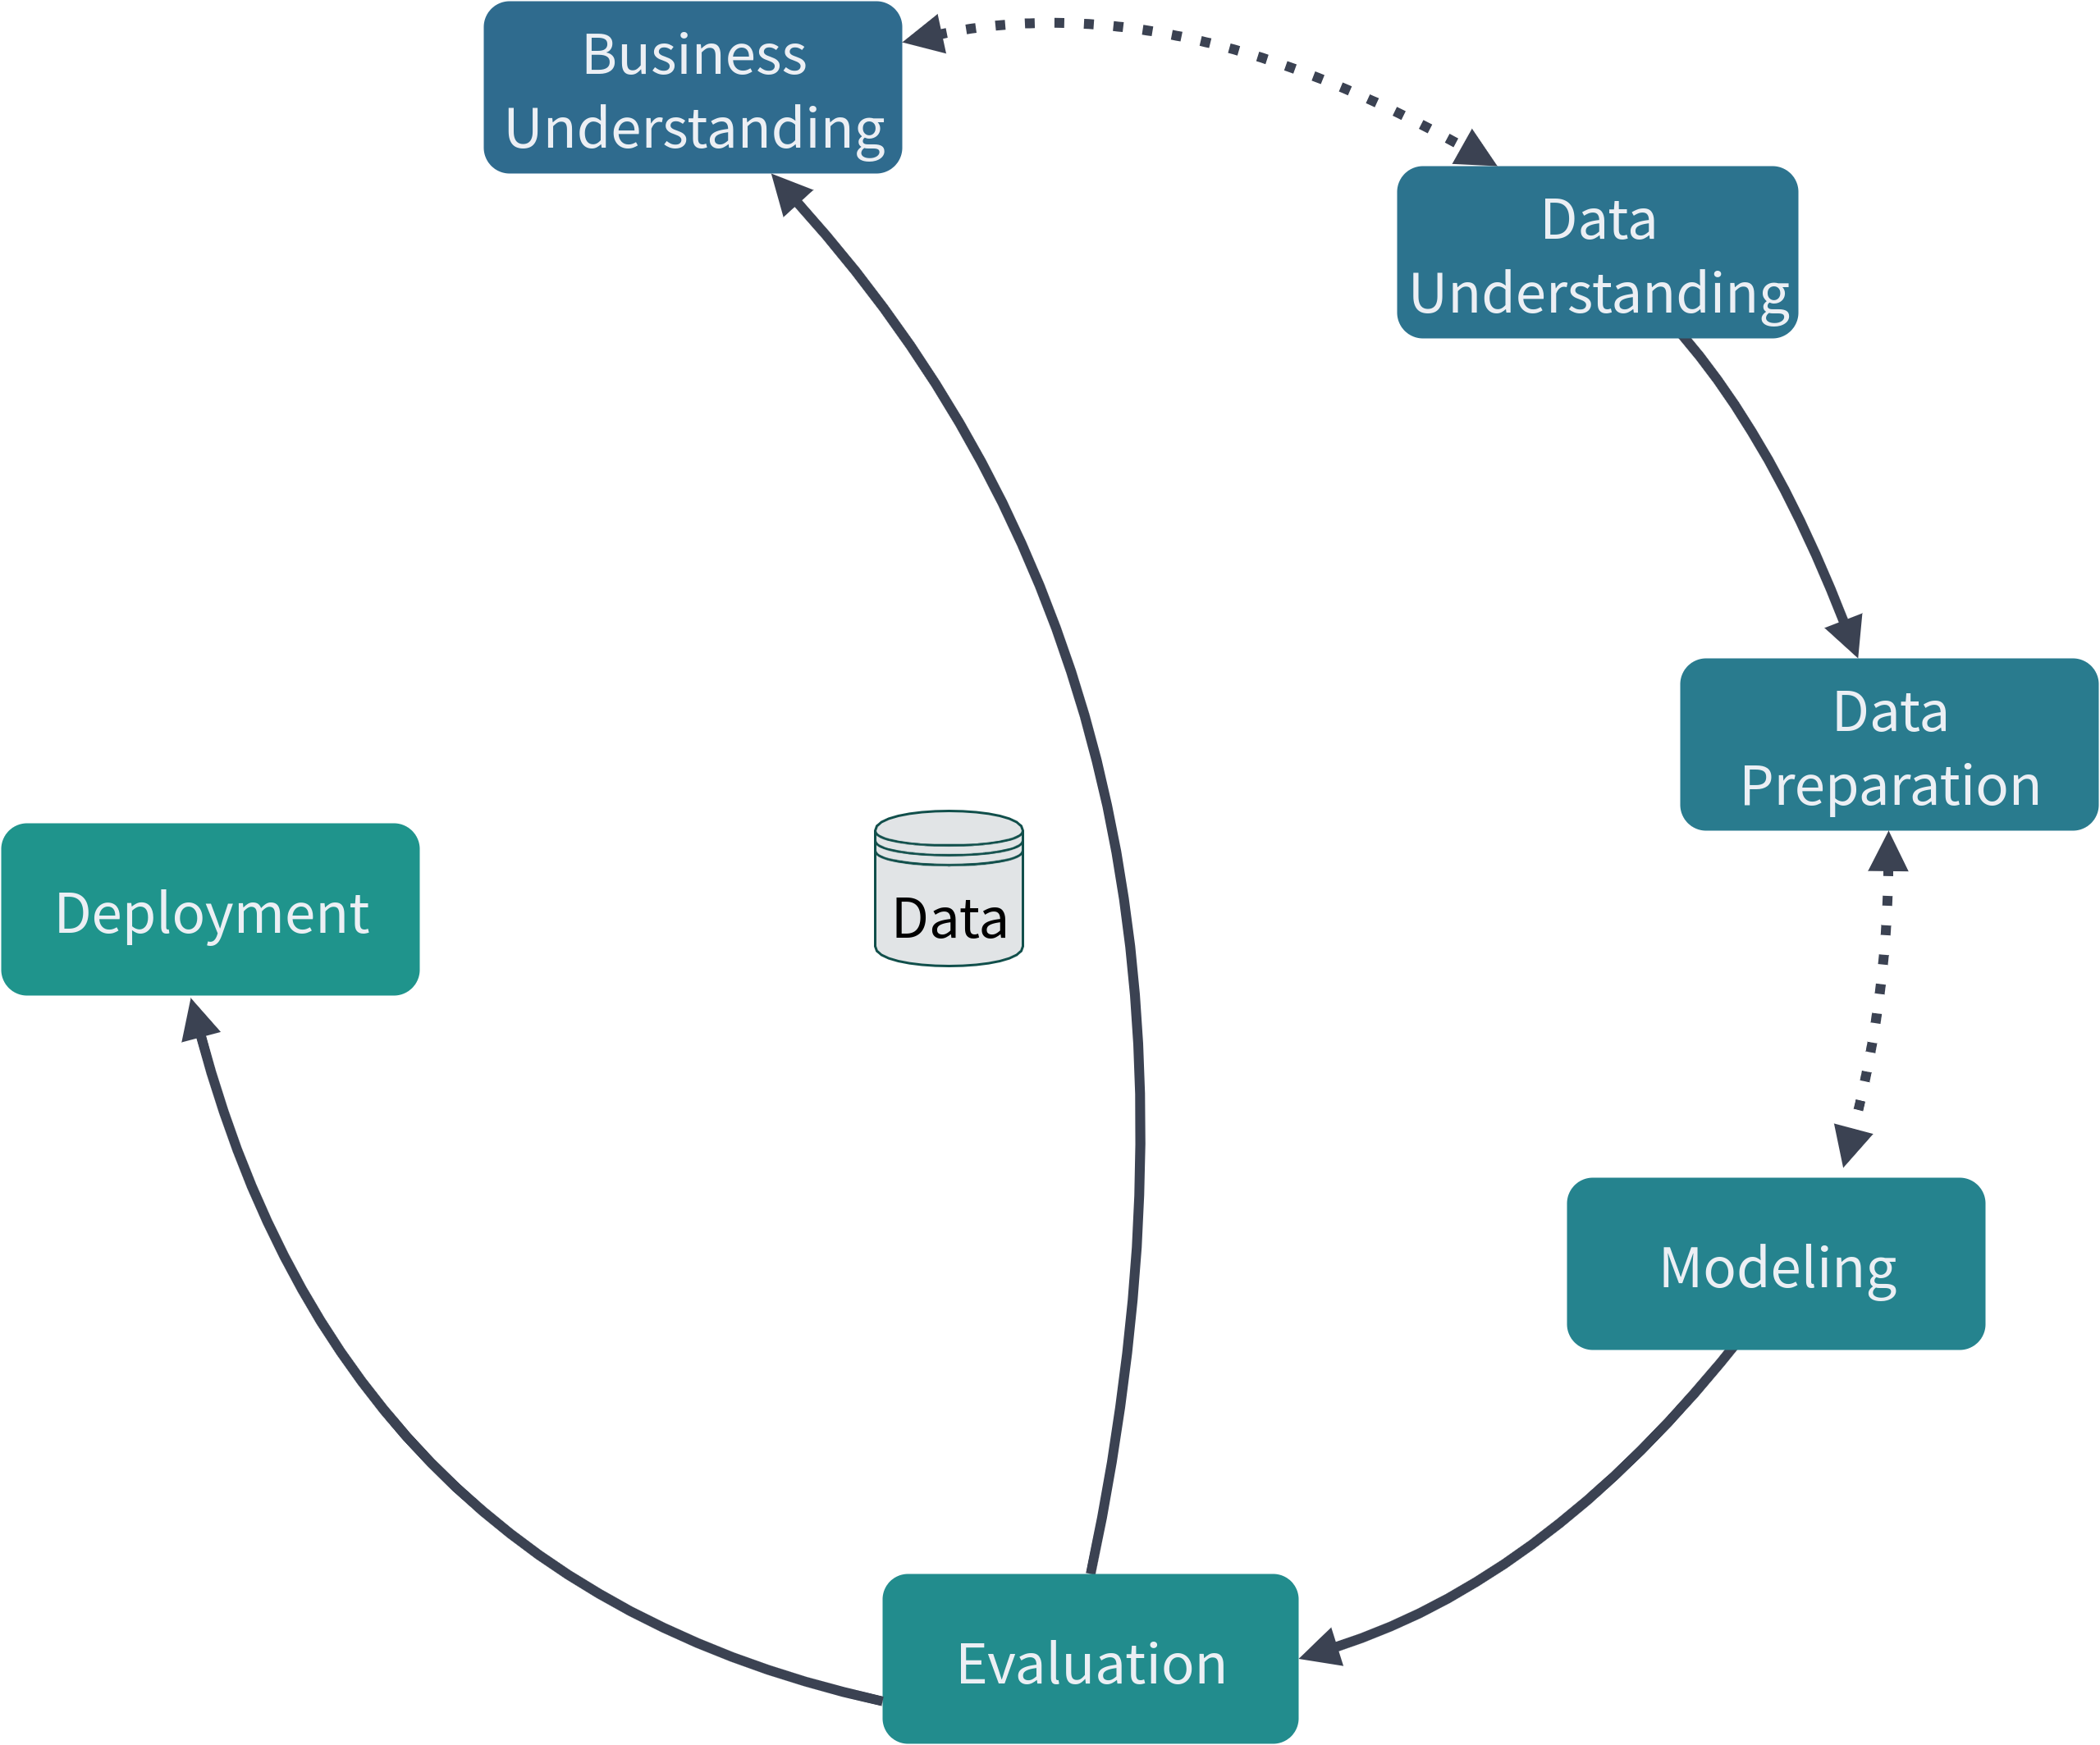
\includegraphics[width=0.8\textwidth]{figures/crisp_dm}
        \end{center}
        \caption{Phasen des CRISP-DM Prozessmodells (in Anlehnung an \cite{wirth_crisp-dm_2000})}
        \label{ch1:fig:crisp}
    \end{small}
\end{figure}

In der ersten Phase \IT{Business Understanding} werden die Ziele und Anforderungen aus der Problembeschreibung abgeleitet, dies erfolgt in \autoref{ch:problem}.

Mittels Background Subtraction werden die Daten für ein Klassifikationsmodell vorbereitet.
Diese zwei Komponenten sind Augenmerk des Konzepts und werden in \autoref{ch:concept} beschrieben \IT{(Data Perparation \& Modeling)}.

In \autoref{ch:eval} erfolgt die Evaluation des Konzeptes.
Zur Evaluation wird ein Prototyp im Maßstab $1:100$ nachgebaut.
Anhand der Aufnahmen des Prototypes erfolgt in diesem Kapitel eine konkrete \IT{Data Understanding} Phase.
Anhand der Ergebnisse der Evaluation werden die Anforderungen an das Konzept diskutiert und die Forschungsfragen beantwortet.

Nach der Evaluation kann das Modell in der Produktion eingesetzt werden \IT{(Deployment)}, dieser Schritt ist jedoch nicht mehr Teil dieser Arbeit.

Zum Abschluss dieser Arbeit erfolgt eine kurze Zusammenfassung und ein Ausblick in \autoref{ch:final}.

% Die Stabilität des Ansatzes wird getestet, indem reale Wettereinwirkungen wie Regen und Nebel simuliert werden.
% Obwohl der Rotmilan nur tagsüber fliegt, wird das Kleinvieh auch nachts aufgescheucht.
% Deshalb müssen Bodenbewirtschaftungsereignisse auch nachts erkannt werden.


% Business Understanding: Aufbau am Windrad
% Data Understanding: Kamerawahl
% Data Preperation: BGs + ROI extraktion
% Modelling: EFN
% Evaluation: Metriken+Ergebnisse